% !TEX root = ba_doc.tex
\begin{markdown}

# Results

## User Interface

The user interface was designed to provide students with the familiar look and feel of a native mobile application. We chose a minimalistic design approach. The focus was on displaying relevant information without any distracting noise or clutter.

The mockups were made so that both of us could work independently and no design decisions had to be made on the go (see Figure \ref{fig:MobileMockups}). It was important to us to have a consistent design throughout the application.

\begin{figure}[H]
  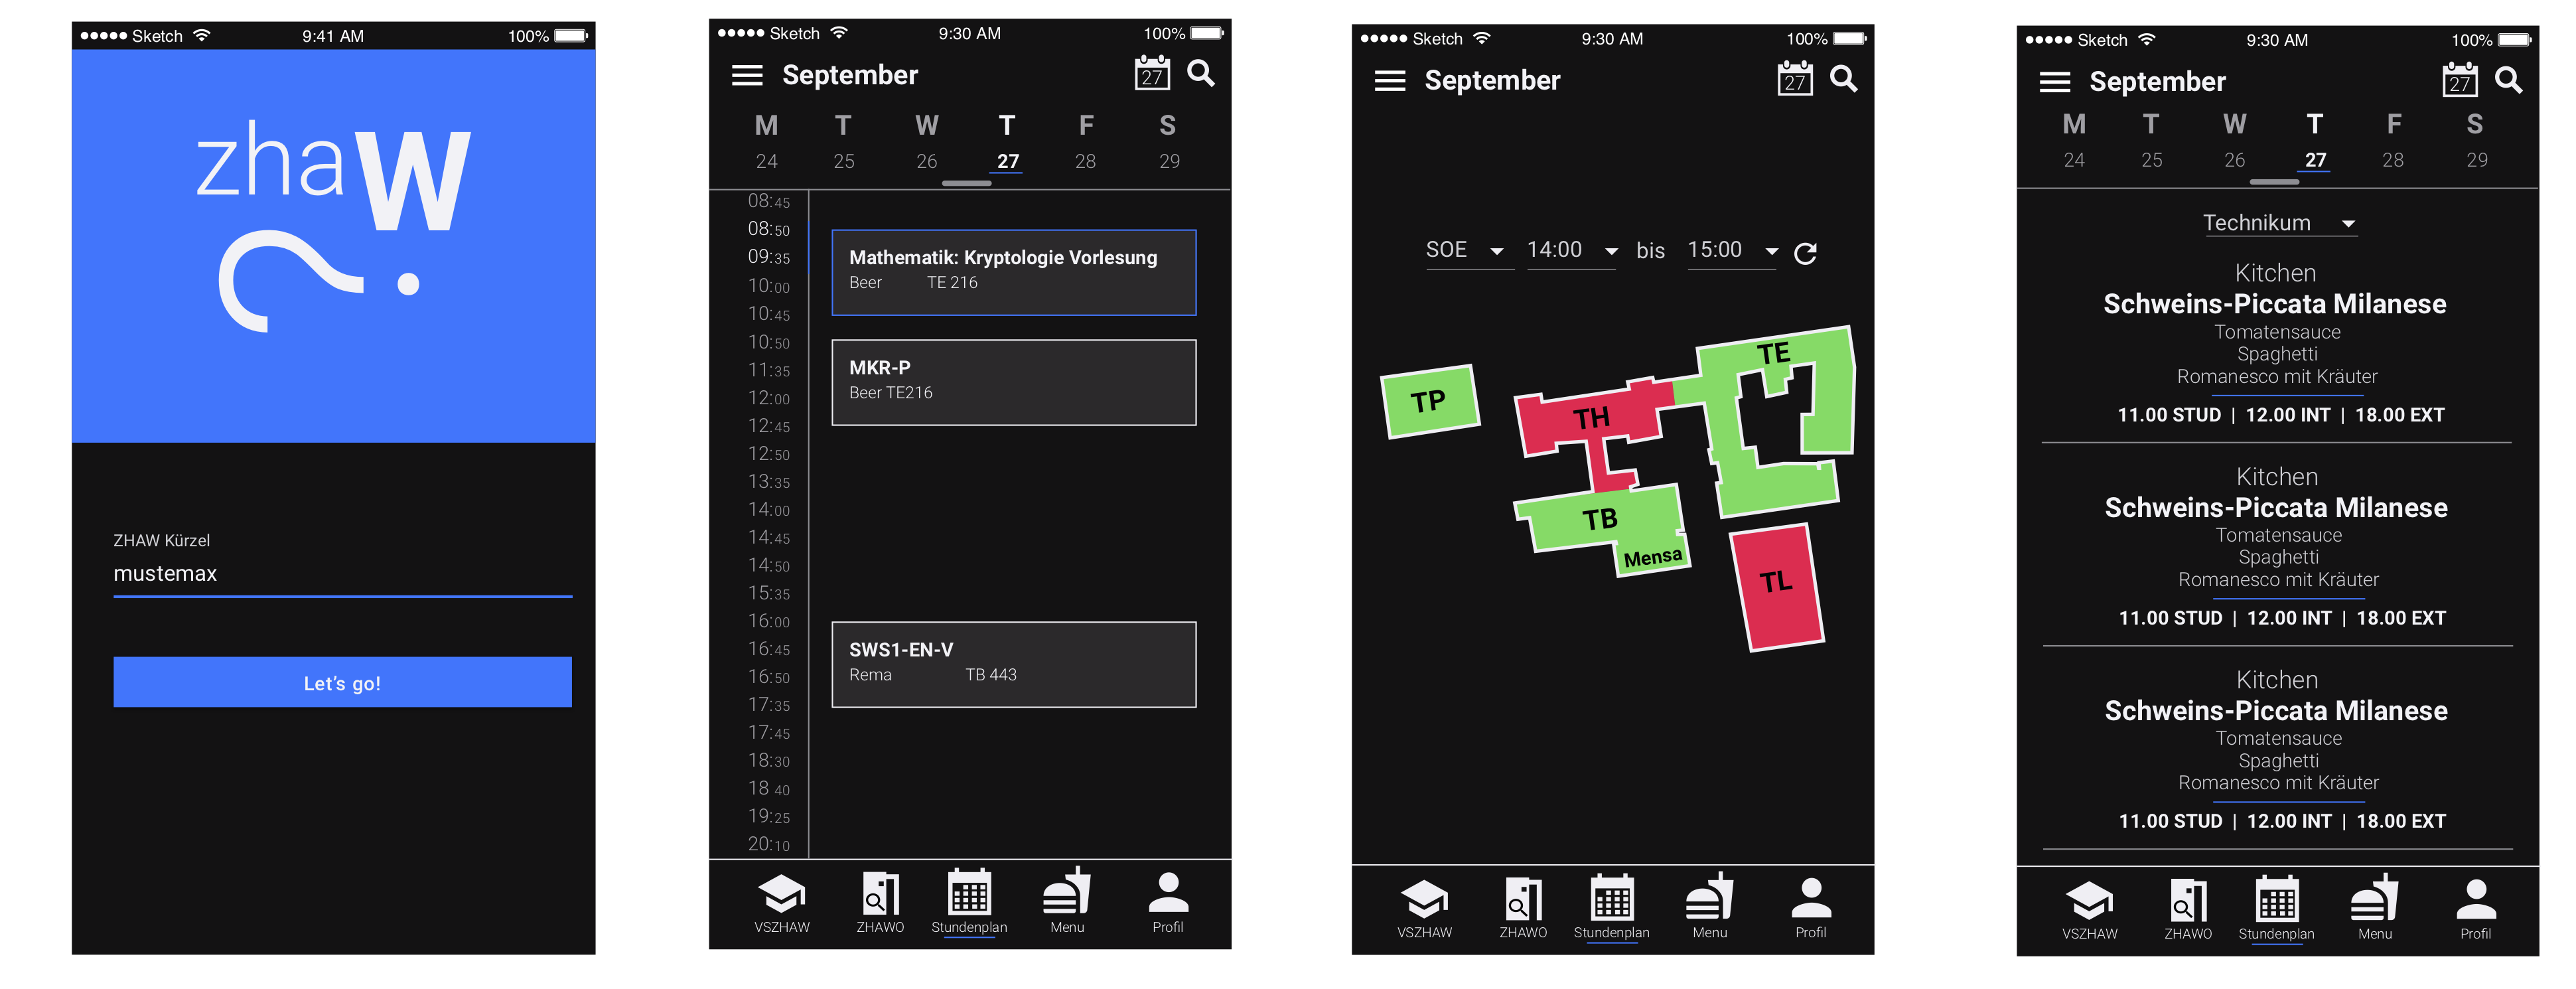
\includegraphics[width=17.75cm, center]{../../Mockups/Mobile_Mockups.png}
  \caption{\textsf{Mobile Mockups}}
  \label{fig:MobileMockups}
\end{figure}

The initial mockups were made with a dark theme. Our first user feedback on the design was very positive, but we learned that most users preferred a light theme over our dark theme. We decided to changed the default theme, whilst still leaving the option for users to change to the dark theme if preferred.

\bigskip

\begin{figure}[H]
  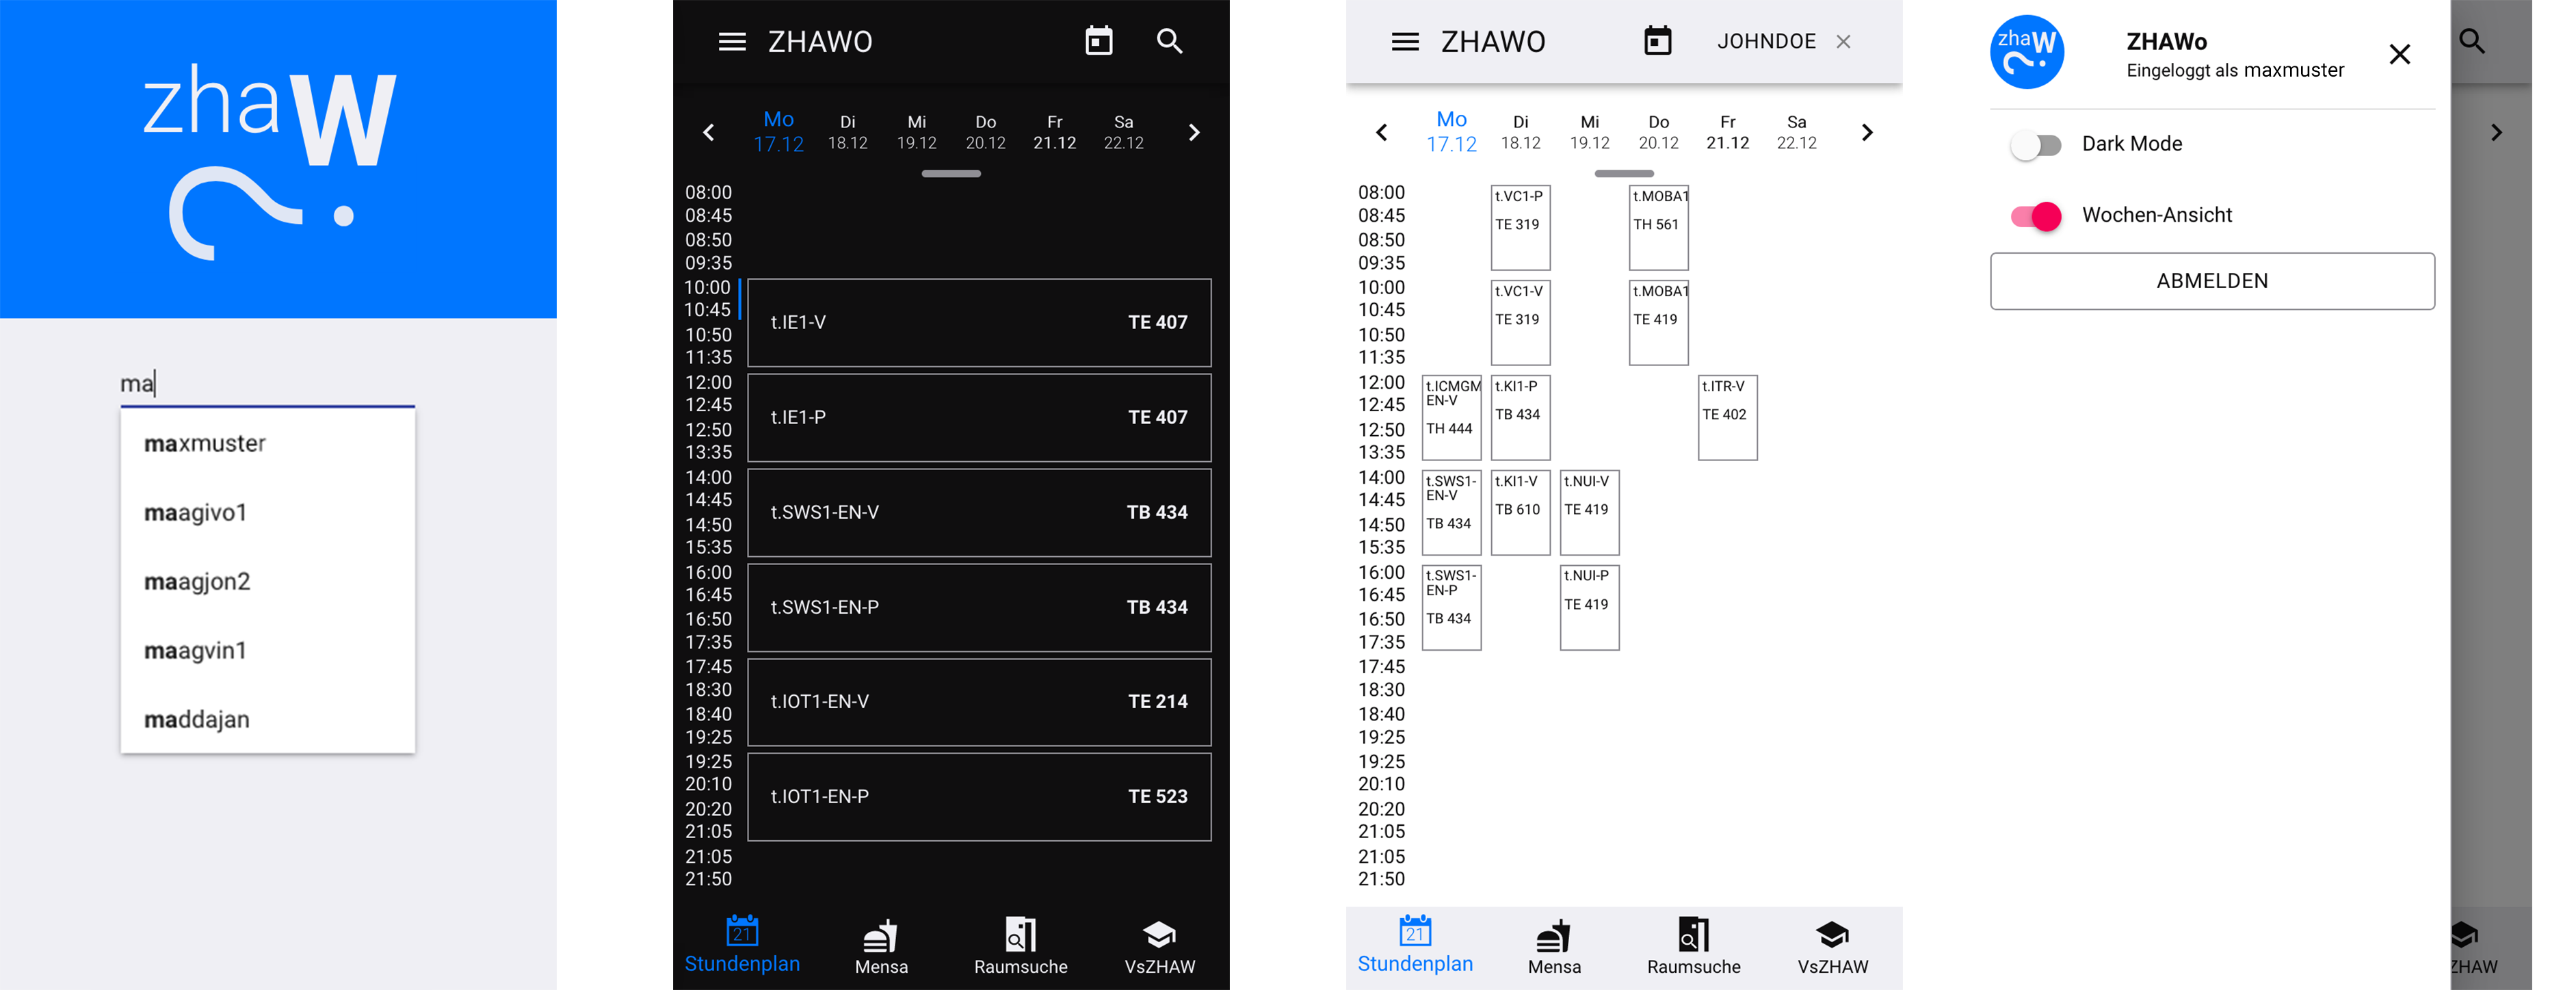
\includegraphics[width=16.5cm, center]{../../Mockups/screenshots.png}
  \caption{\textsf{Mobile Screenshots}}
\end{figure} 

\end{markdown}

